\subsection{Void Swelling}
A correlation for the volumetric void swelling of the cladding was given. We assumed the swelling to be isotropic and therfore the radial expansion is $\frac{1}{3}$ of the volumetric expansion.
Figure \ref{fig:void_swelling} shows the swelling of the cladding along the axial direction.
We can see that, as expected, the swelling is only contained within a range of temperature: too low and no swelling, too high and the mobility is high enough that recombination prevails.

\begin{figure}[H]
\centering
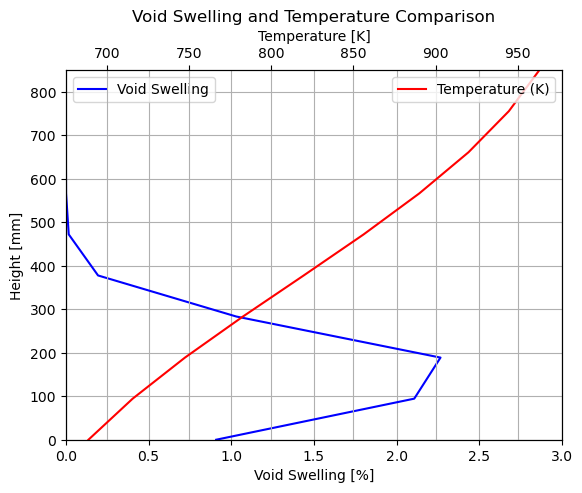
\includegraphics[width=0.8\textwidth]{void_swell.png}
\caption{Cladding swelling due to void formation.}
\label{fig:void_swelling}
\end{figure}
